\section{Verallgemeinerung von Klauseln}
\label{sec:ana:generalize}

generell erweiterung auf bitbreite: bei addierer sehr erfolgreich\\
geht für die vollständige kompressionsfunktion (auch ein modul)

Auf Addierer eingehen: zusätzliche Submodule
\begin{figure}[!h]
  \centering
  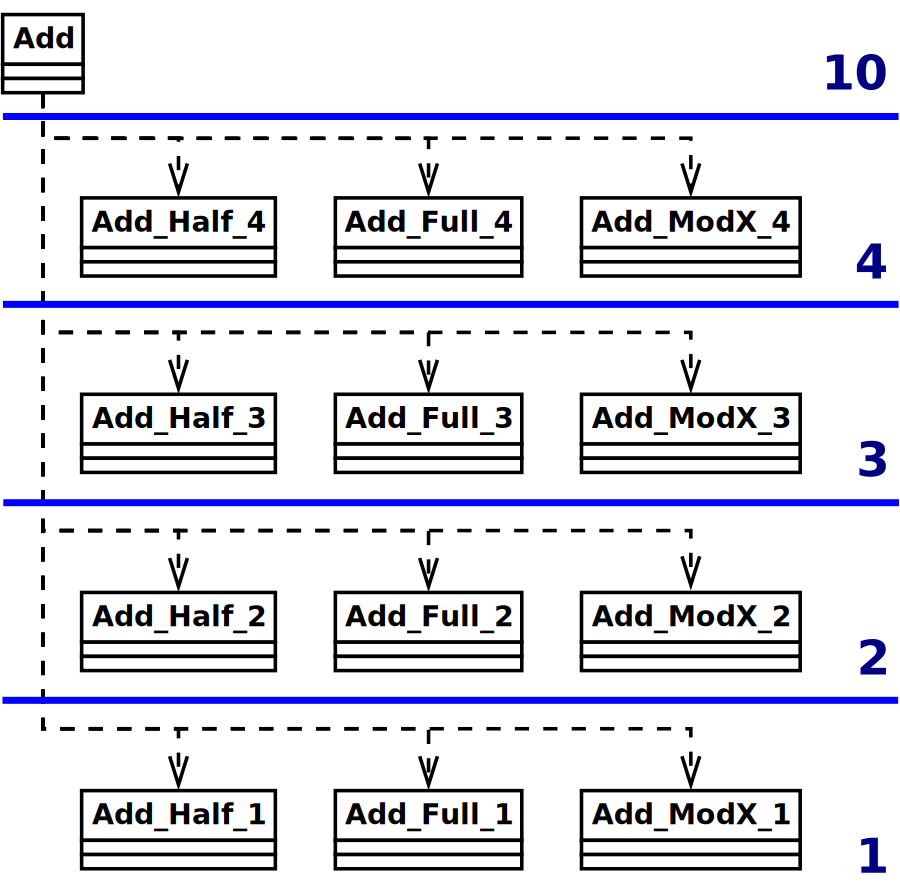
\includegraphics[scale=0.265]{images/module_add}
  \caption{Ergänzte Module von \glos{sha256}}
  \label{fig:sha256_module_add}
\end{figure}


bei kompressionsfunktion: erweiterung auf runden: mit clausechecker prüfen

\TODO{erledigen}